\title{Comment on Jonas et. al paper}
\author{Charles Zheng and Qingyuan Zhao}
\date{\today}

\documentclass[12pt]{article} 

% packages with special commands
\usepackage{amssymb, amsmath}
\usepackage{epsfig}
\usepackage{array}
\usepackage{ifthen}
\usepackage{color}
\usepackage{fancyhdr}
\usepackage{graphicx}
\usepackage{mathtools}
\usepackage{csquotes}
\definecolor{grey}{rgb}{0.5,0.5,0.5}

\begin{document}
\maketitle

\newcommand{\tr}{\text{tr}}
\newcommand{\E}{\textbf{E}}
\newcommand{\diag}{\text{diag}}
\newcommand{\argmax}{\text{argmax}}
\newcommand{\Cov}{\text{Cov}}
\newcommand{\Var}{\text{Var}}
\newcommand{\argmin}{\text{argmin}}
\newcommand{\Vol}{\text{Vol}}
\newcommand{\comm}[1]{}

\begin{figure}[h]
\centering
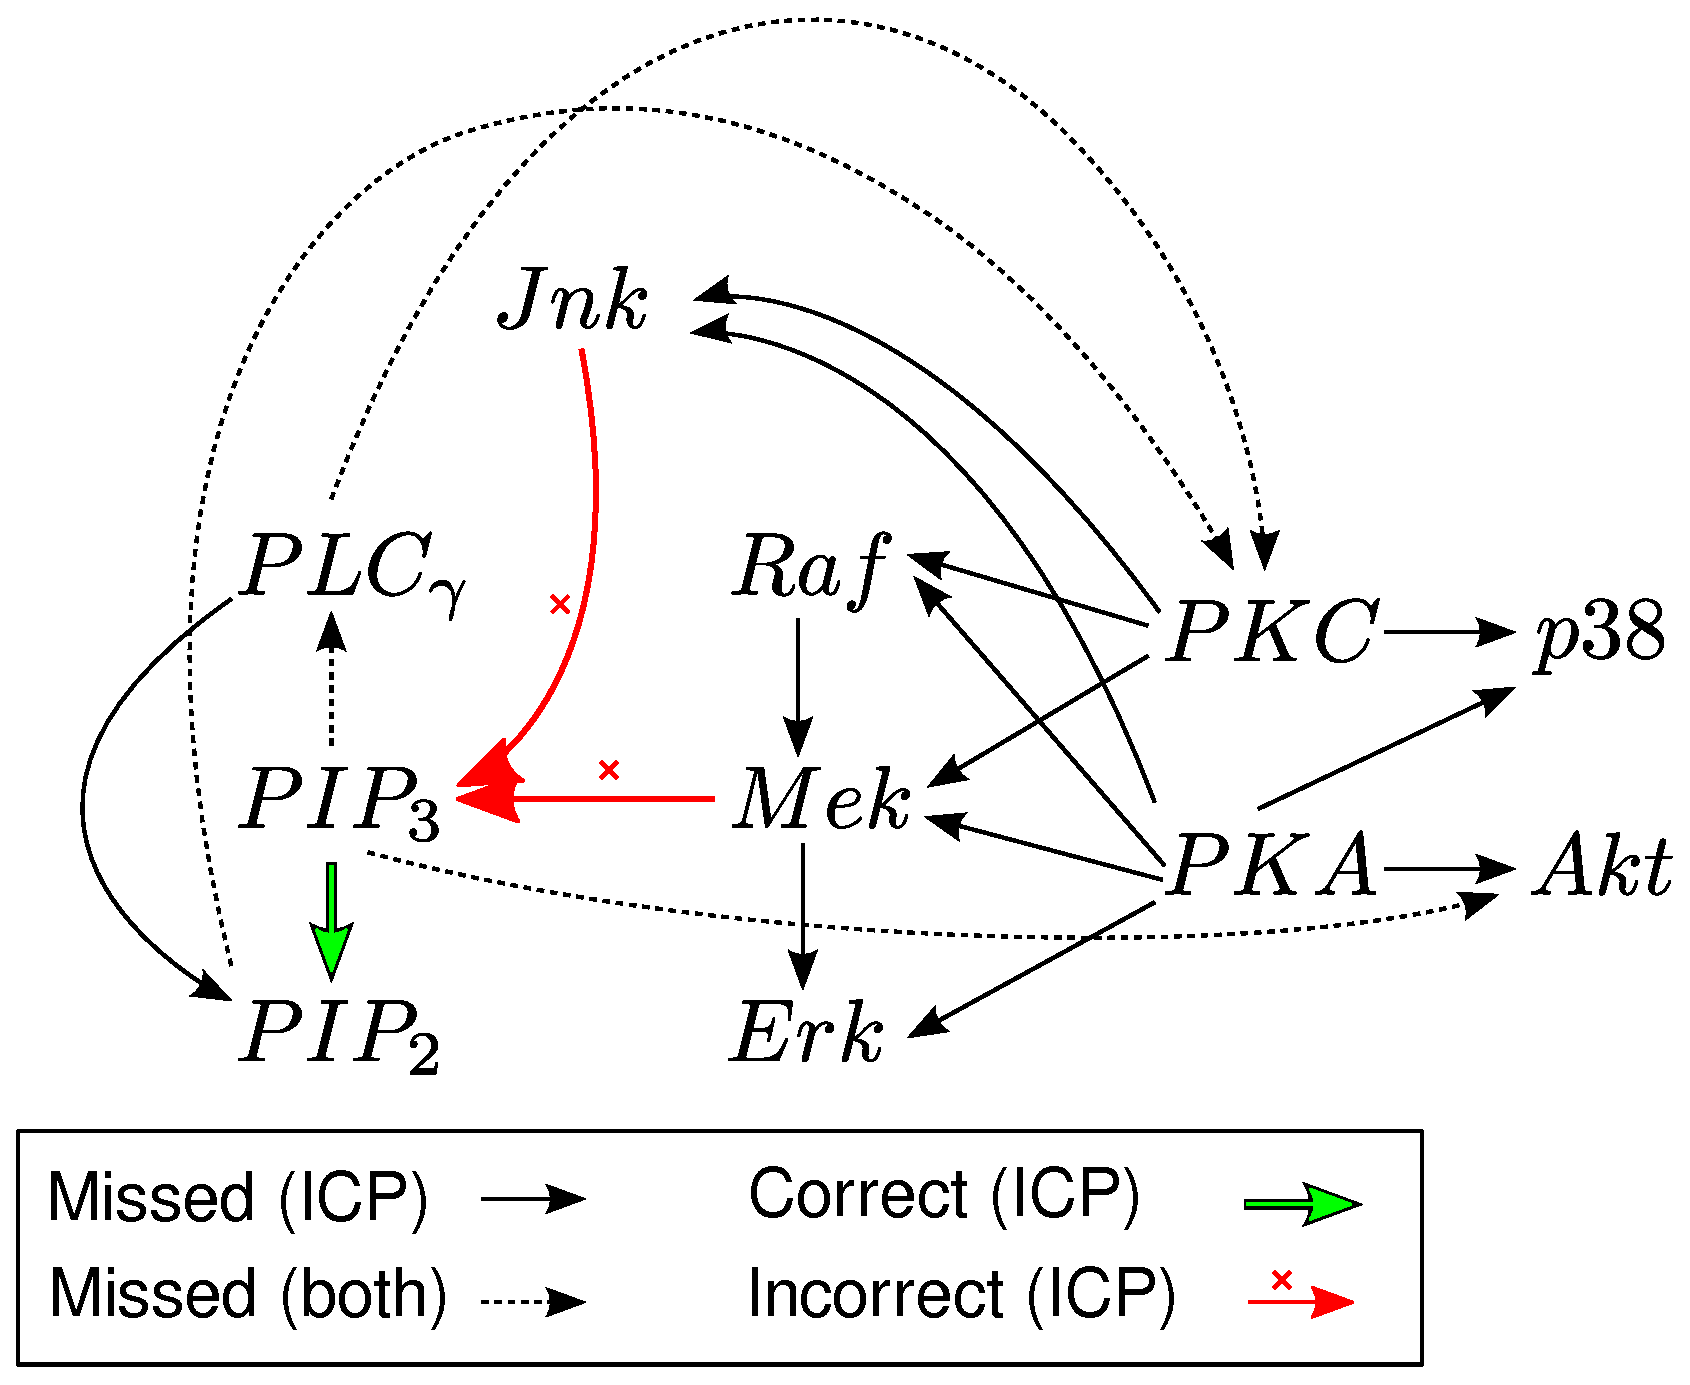
\includegraphics[scale = 0.5]{drawing2legend.eps}
\end{figure}

\begin{figure}[h]
\centering
  \begin{tabular}{|c|c|}
    \hline
    \textbf{Issues} & \textbf{ICP's behavior} \\
    \hline
    Intervene on $Y$ (or a missing cause) &
    $\underset{\emptyset}{\bigcap}$ \\
    \hline
    Non-linear, non-additive, and/or heteroskedastic &
    $\underset{\emptyset}{\bigcap}$ \\
    \hline
    Not enough interventions &
    \textcolor{red}{False positives}$^1$ \\
    \hline
    Small sample size &
    $\emptyset$ \\
    \hline
    Left out a confounder & $\underset{\emptyset}{\bigcap}$ \\
    \hline
    Left out an unconfounding predictor & okay  \\
    \hline
    Misspecified noise model$^2$ & \textcolor{red}{False positives}\\\hline
  \end{tabular}
\end{figure}


\end{document}



